\documentclass{beamer}

\usepackage[utf8]{inputenc}
\usepackage{default}
\usepackage{ulem}
\usepackage{graphicx}
\usepackage[frenchb]{babel}

\title{Recherche Documentaire}
\author{Jean-Baptiste Dalle \& Romain Gaborieau}
\date{23 mars 2015}

\usetheme{Warsaw}

\begin{document}

\maketitle

\begin{frame}
\frametitle{Introduction}


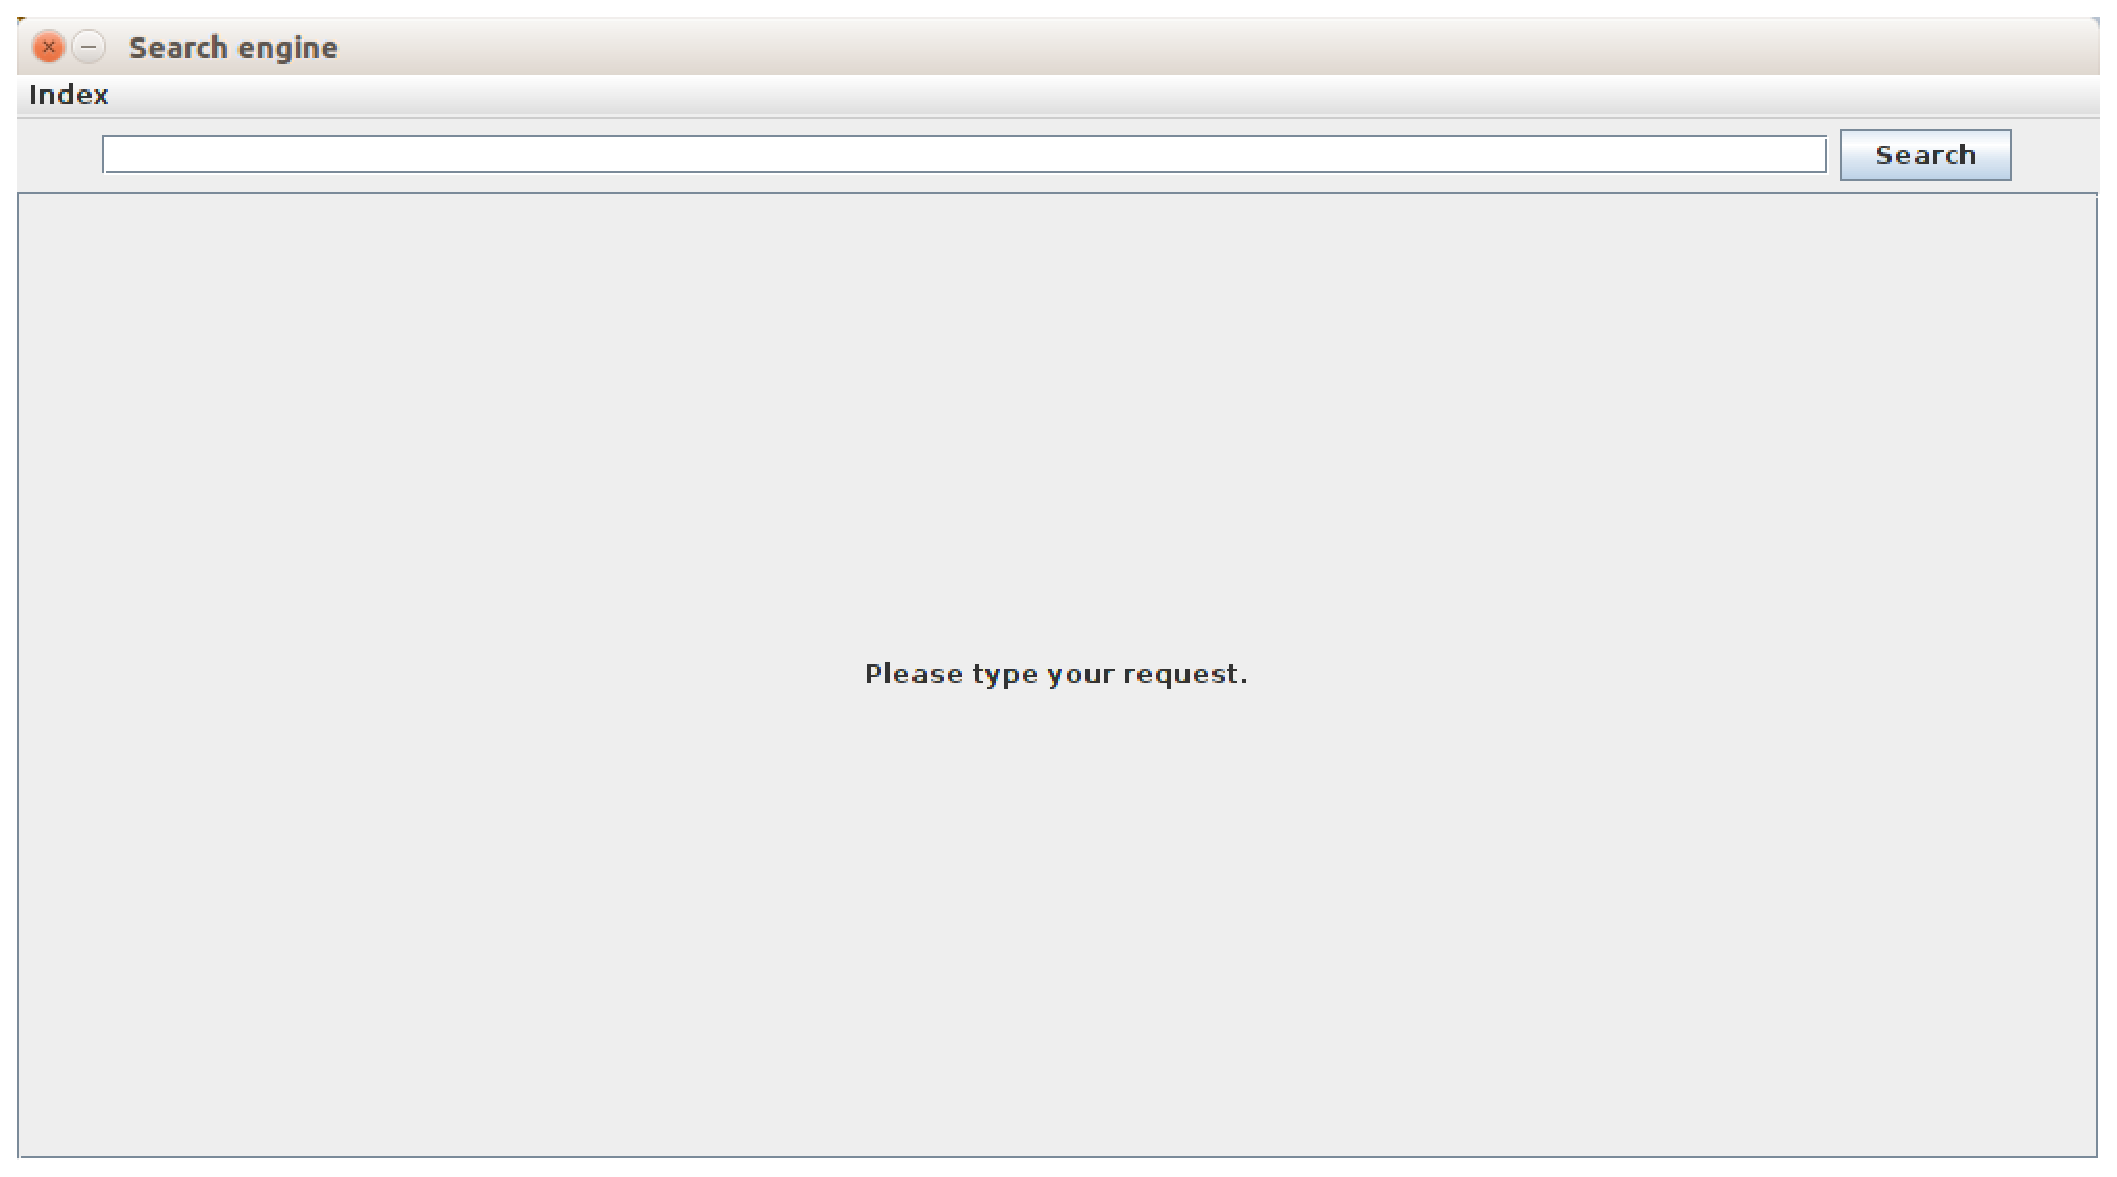
\includegraphics[width=1\linewidth]{img/home}

 
\end{frame}

\begin{frame}
\frametitle{Introduction}


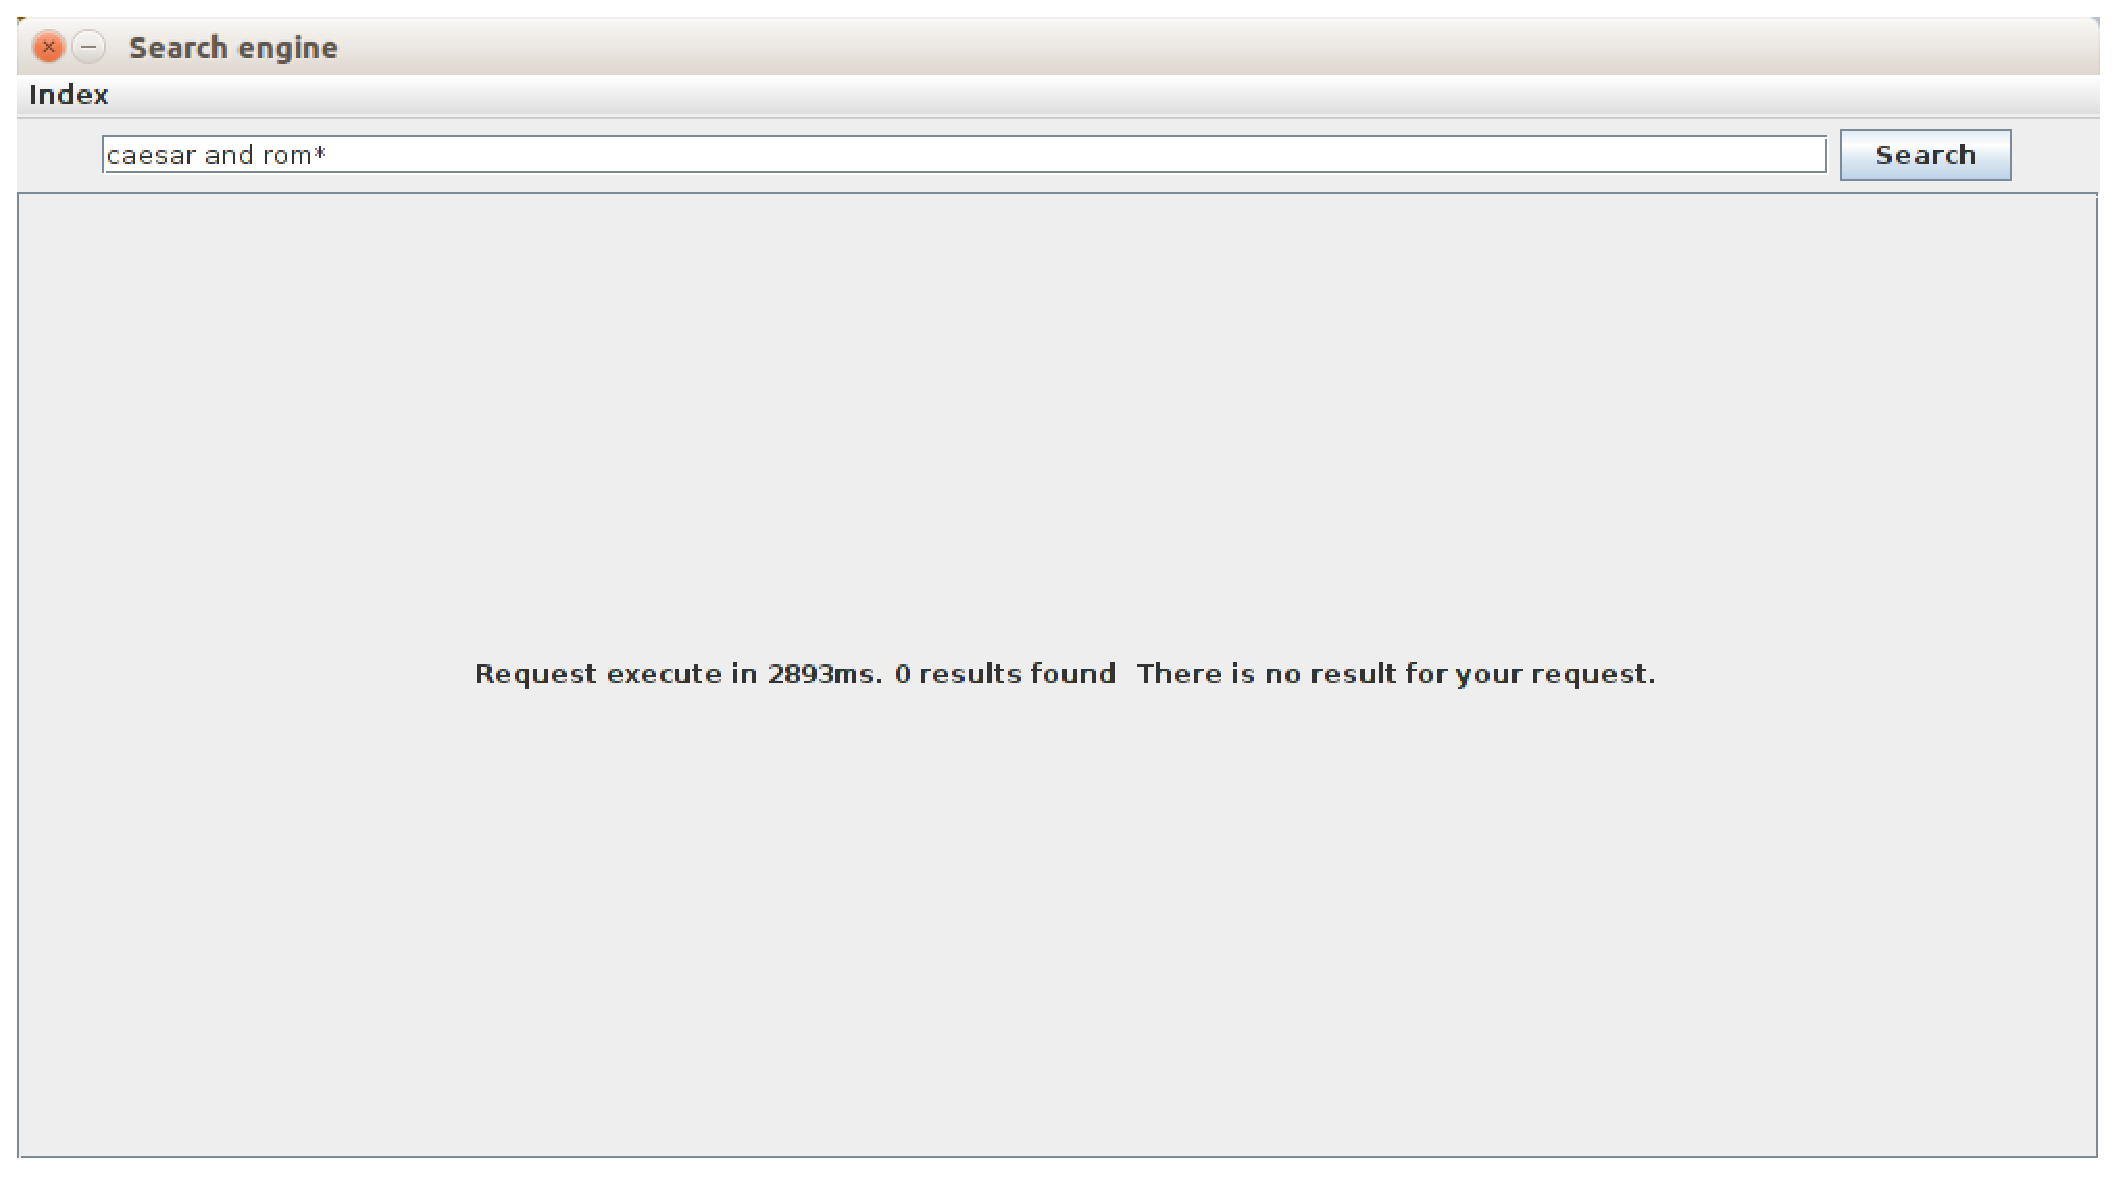
\includegraphics[width=1\linewidth]{img/notfound}

 
\end{frame}

\begin{frame}


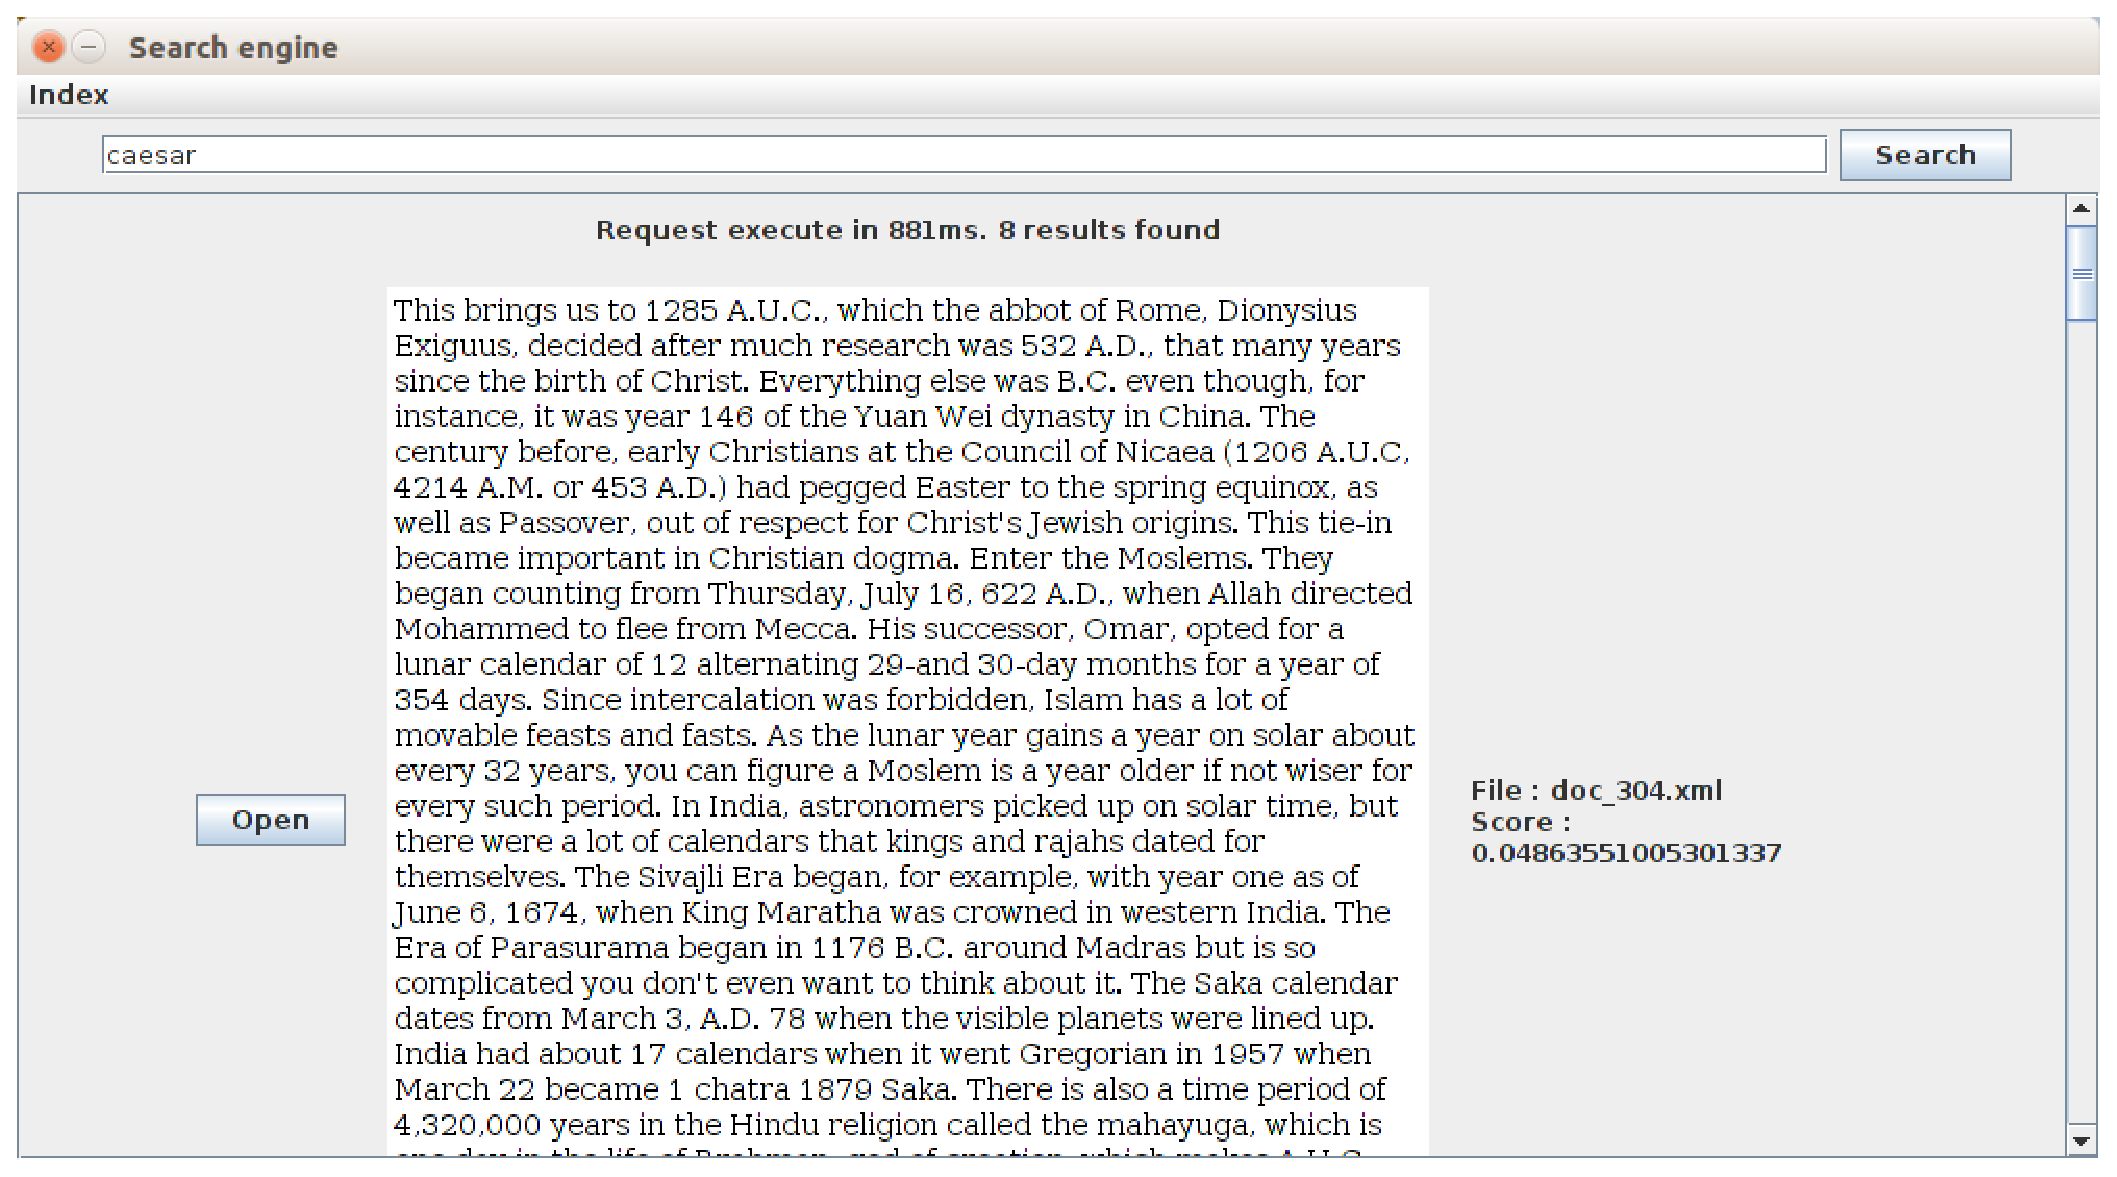
\includegraphics[width=1\linewidth]{img/found}
\frametitle{Introduction}

 
\end{frame}

\begin{frame}

\frametitle{Corpus}

\begin{itemize}
 \item Un document par fichier
 \item Document au format XML
 \item Prise en compte uniquement de la partie "corps du texte"
\end{itemize}

 
\end{frame}

\begin{frame}

\frametitle{Indexation}
\framesubtitle{Sa forme}

\begin{itemize}
 \item Plusieurs mod\`eles possibles
 \item Choix du mod\`ele vectoriel
\end{itemize}


\begin{description}
 \item["caesar"] $\rightarrow$ D1 \{3, 56\} $\rightarrow$ D3 \{7\}
 \item["world"] $\rightarrow$ D6 \{1, 5, 6\} $\rightarrow$ D3 \{8\} $\rightarrow$ D8 \{4\}
\end{description}
 
\end{frame}

\begin{frame}

\frametitle{Indexation}
\framesubtitle{Les stopwords et la racinisation}

\begin{itemize}
 \item Suppression des caract\`eres sp\'eciaux
 \item Suppression des mots non sp\'ecifiques
 \item R\'eduction des mots \`a leur racine
\end{itemize}

\begin{block}{Performances}
 L'indexation peut prendre un certain temps. Dans le cadre du projet, il n'est lanc\'e qu'au premier d\'emarrage de l'application ou sur demande.
\end{block}

 
\end{frame}

\begin{frame}

\frametitle{Les requ\^etes}
\framesubtitle{Leur format}

\begin{exampleblock}{Exemple}

caesar is the king \textit{and} dog \textit{not} world

\end{exampleblock}

\begin{itemize}
 \item Une requ\^ete est consid\'er\'ee comme un document \`a part enti\`ere
 \item D\'ecoupage en sous-requ\^etes
 \item Le m\^eme proc\'ed\'e de racinisation et de suppression des stopwords est r\'ealis\'e sur chaque sous-requ\^ete
\end{itemize}


 
\end{frame}

\begin{frame}

\frametitle{Les requ\^etes}
\framesubtitle{Les op\'erateurs}

\begin{exampleblock}{Exemple}

caesar is the king \textit{and} dog \textit{not} world

\end{exampleblock}

\begin{exampleblock}{D\'ecoupage}

\begin{description}
\item[] caesar \sout{is the} king 
\item[and] dog 
\item[not] world
\end{description}


\end{exampleblock}

 
\end{frame}

\begin{frame}

\frametitle{Les requ\^etes}
\framesubtitle{Les jokers}

\begin{exampleblock}{Exemple}

caesar is the king \textit{not} rom*

\end{exampleblock}

\begin{itemize}
 \item L'indexation associe toutes les variantes non stemm\'ees \`a leur racine
 \item Utilise les \textit{regex} pour matcher le pattern
 \item \textit{rom*} peut correspondre \`a \textit{roma} comme \`a \textit{roman}
\end{itemize}

 
\end{frame}

\begin{frame}

\frametitle{Les r\'esultats}
\framesubtitle{La pertinence}

\begin{itemize}
 \item Calcul du TF d'un mot dans un document : $ \log_{10}(\frac{nbOccurences}{nbMot}) $
 \item Calcul de l'IDF d'un mot dans le corpus : $ \log_{10}(\frac{tailleDuCorpus}{nbOccurences}) $
 \item Le TF-IDF d'un mot dans un document est alors calcul\'e \`a partir de ces donn\'ees
\end{itemize}

 
\end{frame}

\begin{frame}

\frametitle{Les r\'esultats}
\framesubtitle{La proximit\'e}

\begin{itemize}
 \item Repr\'esentation des documents sous forme de vecteur
 \item Calcul de la proximit\'e gr\^ace au cosinus de Salton
 \item Plus la r\'eponse est proche de 0, plus le document est pertinent
\end{itemize}

 
\end{frame}

\begin{frame}

\frametitle{Les extensions}

\begin{itemize}
 \item Une correction orthographique est propos\'ee
 \item Affichage dans la console
 \item Am\'elioration en s\'electionnant automatiquement une correction?
\end{itemize}

 
\end{frame}

\begin{frame}
 \frametitle{Conclusion}
 
 Avez-vous des questions?
 
\end{frame}



\end{document}
